%-------------------------------------------------------------------------
% Design Project Input/Output Module Description
%-------------------------------------------------------------------------

\clearpage
\section{RF Input Module}
\label{sec-input-rf}

This input module enables your IoT device to send and receive radio
frequency (RF) signals wirelessly in a \wu{25}{ft} radius. RF control
devices are useful in many applications -- e.g., car security systems,
home security and automation systems, garage door controllers, remote
control fan, remote control toys, remote control industrial use. In an
RF-based control system, an RF transmitter sends signals -- radio waves
in the range of \wu{3}{kHz} to \wu{300}{GHz} -- and an RF receiver
receives the signals and can then act on them. In this module, you will
use a 4-button keyfob RF remote to send \wu{315}{MHz} signals to an RF
receiver connected to your Arduino, which can then act on the signal.

A sample circuit is shown below to get you started. If you look closely
at the RF receiver module, you will see that it has seven pins total.
Besides power and ground, the D0, D1, D2, and D3 pins are signal pins
corresponding to the four buttons on the keyfob RF remote; VT is a
special pin that is true if any button is pushed and false if none are
pushed. Connect D0, D1, D2, and D3 to the analog input pins on the
Arduino. The 4-button keyfob RF remote requires no assembly or
connectivity. It has four buttons that are labeled "A", "B", "C", and
"D". Pressing any of these transmits a \wu{315}{MHz} radio wave command
to be picked up by the RF receiver.

The example Arduino code shown below will read which button you have
pressed on the remote, and then print the output on the serial monitor,
similar to how we printed the analog reading from the grayscale sensor
in Lab~2. The printout refreshes every \wu{100}{ms}. After setting up the
circuit and programming the Arduino, open the serial monitor and try
pressing each button on the RF remote. You should see each letter
detected by the Arduino displayed on the serial monitor. Try to see how
far away you can move with the RF remote while still successfully
receiving the signal!

\vspace{0.1in}
\begin{minipage}[t]{0.49\tw}

  \vspace{0.1in}
  
\includegraphics[width=\tw]{rf-remote.jpg}

  \vspace{0.1in}
  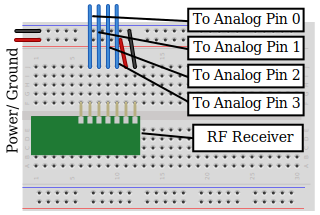
\includegraphics[width=\tw]{input-rf-annotated.svg.pdf}

\end{minipage}
\hfill
\begin{minipage}[t]{0.49\tw}
  \vspace{0.1in}
  \begin{Verbatim}[gobble=3,fontsize=\small]
    int pin_RF_A = 3;
    int pin_RF_B = 6;
    int pin_RF_C = 7;
    int pin_RF_D = 10;

    void setup() {
      pinMode( pin_RF_A, INPUT );
      pinMode( pin_RF_B, INPUT );
      pinMode( pin_RF_C, INPUT );
      pinMode( pin_RF_D, INPUT );
      Serial.begin(9600);
    }

    void loop() {

      // Read RF input on each pin

      int A = digitalRead( pin_RF_A );
      int B = digitalRead( pin_RF_B );
      int C = digitalRead( pin_RF_C );
      int D = digitalRead( pin_RF_D );

      // Print the letter if the input is detected.
      // Otherwise, print '-' if nothing is detected.

      if (A) Serial.print("A"); else Serial.print("-");
      if (B) Serial.print("B"); else Serial.print("-");
      if (C) Serial.print("C"); else Serial.print("-");
      if (D) Serial.print("D"); else Serial.print("-");

      // After checking all four inputs, make a new line.

      Serial.println();

      // Loop every 100ms.

      delay(100);
    }
  \end{Verbatim}
\end{minipage}
\vspace{0.1in}

%Questions:
